\begin{figure}[htbp]
\centering
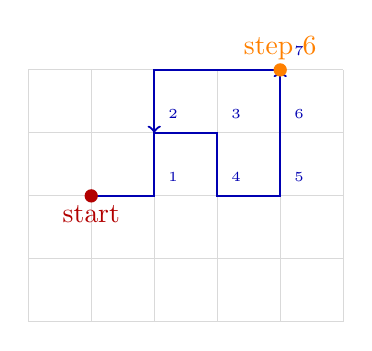
\begin{tikzpicture}[scale=0.8]
  \draw[gray!30,thin] (0,0) grid[step=1] (5,4);
  \draw[blue!70!black,thick,->] (1,2)--(2,2)--(2,3)--(3,3)--(3,2)--(4,2)--(4,3)--(4,4);
  \draw[blue!70!black,thick,->] (4,4)--(3,4)--(2,4)--(2,3);
  \fill[red!70!black] (1,2) circle (3pt) node[below] {start};
  \fill[orange] (4,4) circle (3pt) node[above] {step 6};
  \foreach \x/\y/\s in {2/2/1, 2/3/2, 3/3/3, 3/2/4, 4/2/5, 4/3/6, 4/4/7} {
    \node[font=\tiny,blue!70!black] at (\x+0.3,\y+0.3) {\s};
  }
\end{tikzpicture}
\caption{Random walk on a grid: at each step, move to a uniformly random neighboring vertex.}
\label{fig:random_walk}
\end{figure}
